Порождающие модели --- современное и быстро развивающееся направление работы с данными, позволяющее создавать искусственные данные и 
наращивать вероятностную массу. Ряд ключевых достижений направления:
\begin{enumerate}
    \item порождающие грамматики \cite{chomsky2002syntactic};
    \item графические вероятностные модели \cite{pearl1988probabilistic};
    \item состязательные порождающие модели \cite{goodfellow2020generative};
    \item диффузионные порождающие модели \cite{song2020score}.
\end{enumerate}
Порождающие модели задают совместное распределение наблюдаемого объекта $x$ и его свойств $y$ --- $p(x,y)$. 
В этом состоит основное различие между порождающими и дискриминирующими моделями $p(y|x)$ \ref{discr_vs_gen}.
\begin{figure}[h]
    \centering
    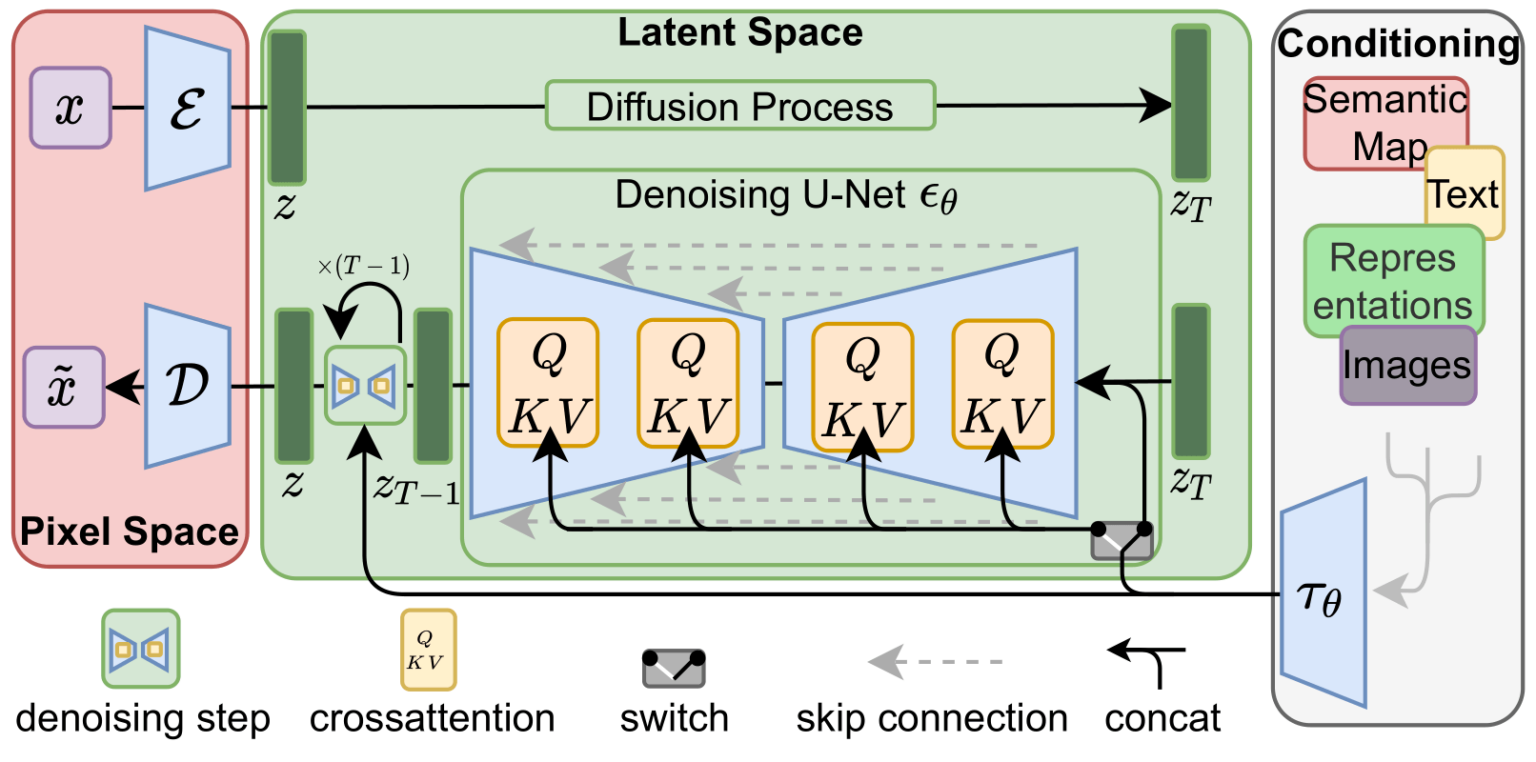
\includegraphics[width=0.6\textwidth]{assets/ml/generation/stable_diffusion.png}
    \caption{Архитектура современной модели Stable Diffusion.}
    \label{discr_vs_gen}
\end{figure}

Порождающие модели используют параметрические модели $p_\theta$ для аппроксимации истинных функций распределений на наборе обучающих данных.
Выбор параметрической функции аппроксимации, как правило, зависит от числа образцов в корпусе данных. Для больших корпусов, как правило, используют нейросети.
Простейшим видом порождающей модели является авторегрессионная модель, использующая предшествующий контекст для предсказания следующего элемента.

\textit{Определение:} \textbf{Авторегрессионные модели} представляют собой класс порождающих моделей,
с вычислимой  вероятностью, выполняющие генерацию с помощью цепи последовательных преобразований:
 \begin{equation}
    p(x^{(1)},\dots,x^{(t)}) = \prod_{t=1}^T p_\theta(x^{(t)}|x^{(1)},\dots,x^{(t-1)})
\end{equation}

Как правило, авторегресионные модели используются для генерации последовательностей, временных рядов и текста.
В то же время с данными, не допускающими однозначного упорядочивания или данными с неравномерным шагом, такой класс
моделей работает недостаточно эффективно.

Для оценки различий между вероятностными распределениями используются \textbf{дивергенции} с набором правил:
\begin{enumerate}
    \item $\forall p,q \in M \rightarrow D(p,q) \ge 0$  
    \item $p=q \leftrightarrow D(p,q) = 0$
    \item $\forall p \rightarrow D(p,p+dp)$ --- положительно определенная квадратичная форма.
\end{enumerate}

В отличие от метрики дивергенции могут быть несимметричны. На практике используются специальный класс $f$-дивергенций, заданных
 матожиданием.

\textit{Определение:} $f$-дивергенцией называется выпуклая функция, удовлетворяющая равенству $f(1)=0$.\:
$$
    D_f(\pi \parallel \rho) = \mathrm E_{\rho(x)} f\left(\frac{\pi(x)}{\rho(x)}\right).
$$

Семейство $f$-дивергенций включает функции:
\begin{enumerate}
    \item дивергенция Кульбака-Лейбнера: $u \ln u $;
    \item обратная дивергенция Кульбака-Лейбнера: $- \ln u$;
    \item дивергенция Йенсена-Шэннона: $\frac{1}{2}\left(u \ln u - (u+1) \ln(\frac{u+1}{2})\right)$.
\end{enumerate}

Нижней вариационной оценкой называется техника максимизации подпирающей границы параметрического распределения $p(\mathbf{x},\mathbf{z})$ вторым $q(\mathbf{x},\mathbf{z})$,
где переменная $\mathbf{z}$ называется скрытой. В аналитической форме нижняя граница записывается как:
\begin{equation}
    \mathcal{L}(\phi,\theta;x) = \mathbb{E}_{z \sim q_\phi(z|x)} \left[\ln \frac{p_{\theta}(x,z)}{q_{\phi}(z|x)}\right].
\end{equation}
Перепишем в виде KL-дивергенции:
\begin{equation}
    \begin{aligned}
        & D_\text{KL}( q_\phi(\mathbf{z}\vert\mathbf{x}) \| p_\theta(\mathbf{z}\vert\mathbf{x}) ) & \\
        &=\int q_\phi(\mathbf{z} \vert \mathbf{x}) \log\frac{q_\phi(\mathbf{z} \vert \mathbf{x})}{p_\theta(\mathbf{z} \vert \mathbf{x})} d\mathbf{z} & \\
        &=\int q_\phi(\mathbf{z} \vert \mathbf{x}) \log\frac{q_\phi(\mathbf{z} \vert \mathbf{x})p_\theta(\mathbf{x})}{p_\theta(\mathbf{z}, \mathbf{x})} d\mathbf{z}\\
        &=\int q_\phi(\mathbf{z} \vert \mathbf{x}) \big( \log p_\theta(\mathbf{x}) + \log\frac{q_\phi(\mathbf{z} \vert \mathbf{x})}{p_\theta(\mathbf{z}, \mathbf{x})} \big) d\mathbf{z} & \\
        &=\log p_\theta(\mathbf{x}) + \int q_\phi(\mathbf{z} \vert \mathbf{x})\log\frac{q_\phi(\mathbf{z} \vert \mathbf{x})}{p_\theta(\mathbf{z}, \mathbf{x})} d\mathbf{z} \\
        &=\log p_\theta(\mathbf{x}) + \int q_\phi(\mathbf{z} \vert \mathbf{x})\log\frac{q_\phi(\mathbf{z} \vert \mathbf{x})}{p_\theta(\mathbf{x}\vert\mathbf{z})p_\theta(\mathbf{z})} d\mathbf{z} \\
        &=\log p_\theta(\mathbf{x}) + \mathbb{E}_{\mathbf{z}\sim q_\phi(\mathbf{z} \vert \mathbf{x})}[\log \frac{q_\phi(\mathbf{z} \vert \mathbf{x})}{p_\theta(\mathbf{z})} - \log p_\theta(\mathbf{x} \vert \mathbf{z})] &\\
        &=\log p_\theta(\mathbf{x}) + D_\text{KL}(q_\phi(\mathbf{z}\vert\mathbf{x}) \| p_\theta(\mathbf{z})) - \mathbb{E}_{\mathbf{z}\sim q_\phi(\mathbf{z}\vert\mathbf{x})}\log p_\theta(\mathbf{x}\vert\mathbf{z}) &
    \end{aligned}.
\end{equation}
Следовательно:
\begin{equation}
    \log p_\theta(\mathbf{x}) - D_\text{KL}( q_\phi(\mathbf{z}\vert\mathbf{x}) \| p_\theta(\mathbf{z}\vert\mathbf{x}) ) = \mathbb{E}_{\mathbf{z}\sim q_\phi(\mathbf{z}\vert\mathbf{x})}\log p_\theta(\mathbf{x}\vert\mathbf{z}) - D_\text{KL}(q_\phi(\mathbf{z}\vert\mathbf{x}) \| p_\theta(\mathbf{z}))
\end{equation}
Таким образом, из неравенства Йенсена получаем: 
$$
    \ln p_\theta(x) \le \mathcal{L}(\phi,\theta;x)
$$
Базовым алгоритмом оптимизации вариационных моделей является EM-алгоритм, состоящий из последовательного обновления
скрытых представлений и максимизации правдоподобия с заданным параметрами.

\textit{Определение:} \textbf{EM-алгоритм} --- алгоритм для нахождения оценок
максимального правдоподобия параметров  вероятностных моделей с скрытыми переменными $\theta$.
Аналитически шаги алгоритма записываются как: 
\begin{itemize}
    \item расчет матожидания при заданном на шаге $t$ параметре $\theta^{(t)}$.
    Шаг обновления:
    \begin{equation}
        Q(\theta| \theta^{(t)}) = \mathbb{E}_{\mathbf{Z} \sim p(\mathbf{Z}|X,\theta^{(t)})} \left[ \log p(\mathbf{X},\mathbf{Z}|\mathbf{\theta})\right]
    \end{equation}
    \item максимизации полученного выражения для нового шага $\mathbf{\theta}^{(t+1)}$: 
    \begin{equation}
        \mathbf{\theta}^{(t+1)} = \text{arg} \max_{\theta} Q(\mathbf{\theta}|\theta^{(t)}).
    \end{equation}  
\end{itemize}
